\subsection{Question 2.1.3}
Finalement, après avoir corrigé les erreurs décrites ci-dessus (notamment la liste initiale pour la sélection des fournisseurs), la figure 9 est reproduite.

\begin{figure}[H]
\centering
\captionsetup{justification=centering}
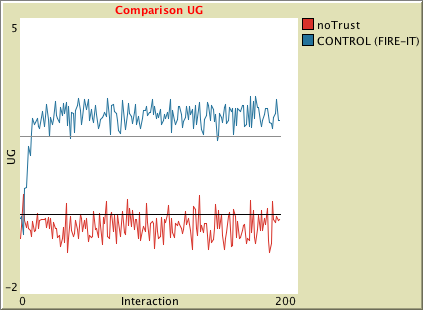
\includegraphics[width=0.3\textwidth]{images/evolutionIT/IT5.png}
\caption{Reproduction de la figure 9 (pour CONTROL = FIRE-IT)}
\label{fig:fig9}
\end{figure}

Le résultat est similaire à celui de l'article à la seule différence près que la courbe croît (et donc se stabilise) plus vite que celle d'origine. Ce phénomène est vient peut-être du fait que les agents ont tendance à passer à l'exploitation plus vite. Deux facteurs peuvent causer ceci : le rayon des agents est trop petit (pas assez de voisins) ou la température décroît trop vite. D'autre part, nous avons également remarqué une variabilité au niveau de la convergence de la courbe entre plusieurs simulations avec des paramètres identiques. Cette différence reste toutefois négligeable.
Pour que le résultat soit plus ressemblant à l'article, c'est-à-dire pour que la courbe soit plus lisse, il est possible de garder tous les UGs obtenue depuis le début de la simulation. Ainsi, on ne viderait pas les listes à chaque \texttt{tick} mais il nous paraissaît plus cohérent d'avoir une moyenne d'UGs obtenue sur les données d'une itération seulement.